%%
%% SEMANTiCS 2026 — Posters & Demos track submission
%% CEUR-ART single-column format, 5 pages incl. references
%% https://ceur-ws.org/HOWTOSUBMIT.html
%%
\documentclass[sigconf,natbib=true]{ceurart}

\usepackage{listings}
\lstset{breaklines=true}
\usepackage{booktabs}
\usepackage{tabularx}
\usepackage{multirow}
\usepackage{graphicx}
\usepackage{hyperref}

\usepackage{tikz}
\usetikzlibrary{shapes.geometric, arrows.meta, positioning, calc, backgrounds, fit, shadows, shapes.misc}

\definecolor{activeblue}{RGB}{220, 240, 255}
\definecolor{activegreen}{RGB}{230, 250, 230}
\definecolor{passivegray}{RGB}{240, 240, 240}
\definecolor{bordergray}{RGB}{120, 120, 130}
\definecolor{textgray}{RGB}{80, 80, 90}
\definecolor{inactivegray}{RGB}{180, 180, 180}
\definecolor{arrowcol}{HTML}{5D6D7E}
\definecolor{phasebg1}{RGB}{230, 240, 250}
\definecolor{phasebg2}{RGB}{255, 250, 235}
\definecolor{phasebg3}{RGB}{255, 240, 245}
\definecolor{boxgray}{RGB}{80, 80, 90}

%% Loosen float placement so figures/tables pack tightly within the
%% 5-page budget instead of fragmenting pages.
\renewcommand{\topfraction}{0.95}
\renewcommand{\bottomfraction}{0.6}
\renewcommand{\textfraction}{0.05}
\renewcommand{\floatpagefraction}{0.95}
\setcounter{topnumber}{3}
\setcounter{totalnumber}{6}

%% Tighten inter-entry spacing in the bibliography (natbib).
\AtBeginDocument{\setlength{\bibsep}{0pt}}

\begin{document}

\copyrightyear{2026}
\copyrightclause{Copyright for this paper by its authors.
  Use permitted under Creative Commons License Attribution 4.0
  International (CC BY 4.0).}

\conference{SEMANTiCS 2026: 22nd International Conference on Semantic Systems,
  September 15--17, 2026, Ghent, Belgium}

\title{AMA-KBQA: An Adaptable Multi-Agent Framework for Generalizable Knowledge Base Question Answering}

\author[1]{Yannic Duan}
[email=yannic.duan@student.kit.edu]
\author[1]{Maximilian Klattig}[email=maximilian.klattig@student.kit.edu]
\author[1]{Maurice Bardenhagen}[email=maurice.bardenhagen@student.kit.edu]
\author[1]{Yuyang Li}[email=yuyang.li@kit.edu]
\author[1]{Tobias Käfer}[email=tobias.kaefer@kit.edu]
\address[1]{Karlsruhe Institute of Technology (KIT), Institute of Applied Informatics and Formal Description Methods (AIFB), Karlsruhe, Germany}

\begin{abstract}
We present \textbf{AMA-KBQA}, a multi-agent framework for
retrieval-augmented generation (RAG) over knowledge graphs that
decouples reasoning by large language models (LLMs) from graph
retrieval through abstract agents, configuration-driven adapters, and
Model Context Protocol (MCP) tool servers. The system requires
\emph{no model training}: onboarding a new knowledge graph reduces to
writing SPARQL wrappers behind an abstract tool interface, and
adopting a stronger LLM is a configuration change. A journal-based
scratchpad keeps reasoning state token-efficient, and a
Lessons-Learned loop distils high-quality traces into few-shot
examples. Across KQAPro and SciQA, the same reasoning core generalises
over a reified encyclopedic graph and a hierarchical scientific graph,
reaching up to 84\% accuracy.
\end{abstract}

\begin{keywords}
  KBQA \sep
  SPARQL \sep
  Large Language Models \sep
  Model Context Protocol \sep
  Knowledge Graphs
\end{keywords}

\maketitle

% Match the abstract/keywords block, which ceurart sets with
% \leftskip = .1\textwidth and \footnotesize
\vspace{-1em}
{\footnotesize
\noindent\hspace*{\dimexpr.1\textwidth-3pt}%
\textbf{Demo} \url{https://purl.archive.org/ama-kbqa-demo}\enspace
\textbf{Code+Video} \url{https://github.com/yannicd03/AMA-KBQA}\par}

\section{Introduction}
Knowledge Base Question Answering (KBQA) is the task of answering
natural-language questions over a structured knowledge base, typically
a Resource Description Framework (RDF) graph queried via SPARQL. KBQA
makes curated graph data accessible to non-experts, and large language
models (LLMs) have become the default instrument for it. Yet LLMs alone suffer from knowledge cutoff,
hallucination, and poor multi-hop reasoning over structured
data~\cite{agrawal2023kg}. Text-to-SPARQL
semantic parsing~\cite{berant2013semantic} and retrieval-augmented
generation (RAG)~\cite{lewis2020retrieval} ground the model in the
graph, but bind the resulting system tightly to one graph's schema and
vocabulary, and state-of-the-art KBQA systems additionally depend on
dataset-specific training, from fine-tuned query
generators~\cite{rony2022sgpt} to trained question
classifiers~\cite{xiong-etal-2024-interactive}. Both forms of coupling
are costly: porting to a new graph or adopting a stronger model means
re-engineering or retraining the pipeline.

This rigidity is particularly painful because deployed knowledge
graphs are not static. Industry-scale graphs evolve continuously as
new domains are onboarded, schemas are refactored, and data sources
are added, replaced, or deprecated~\cite{noy2019industry}; rebuilding
the pipeline for every such change is impractical. What is needed is a
framework that treats both the knowledge graph (KG) and the language
model as swappable components, adapted by configuration rather than
re-implementation.

We introduce \textbf{AMA-KBQA}, a multi-agent framework built around
exactly this requirement. It counters coupling to the graph with an
abstract tool interface: the reasoning core only ever calls typed
graph operations, which each graph implements as deterministic SPARQL
wrappers that insert the tool's parameters into a valid query template
instead of letting the LLM write SPARQL freely. The backbone LLM
itself is a configuration choice. And it requires no dataset-specific
training: a question is answered
by (i)~deterministic \emph{pre-processing} (question classification
and entity extraction), (ii)~\emph{agentic exploration} via typed tool
calls over SPARQL and vector search, and (iii)~\emph{grounded
synthesis} over a scratchpad of verified facts rather than free LLM
generation. On top of these three phases, a Lessons-Learned loop
distils highly rated traces into few-shot examples, so the system
improves over time without fine-tuning.

\section{Related Work}
Text-to-SPARQL systems translate a question directly into a query:
classical semantic parsers learn the mapping from question-answer
pairs~\cite{berant2013semantic}, neural approaches treat SPARQL as a
target language for sequence-to-sequence
models~\cite{soru2017sparql,rony2022sgpt}, and recent work prompts
LLMs to generate SPARQL directly, still with limited
reliability~\cite{meyer2024assessing}. All of these couple the system
to one graph's vocabulary and structure, so a schema change degrades
the learned mapping.
Interactive-KBQA~\cite{xiong-etal-2024-interactive} instead reframes
KBQA as a multi-turn control loop over atomic graph APIs in the spirit
of ReAct~\cite{yao2023react}, paired with a trained BERT question
classifier. We adopt this
agentic stance and extend it for deployability: a configuration-driven
adapter layer ports the same reasoning core to a new knowledge graph
without rewrites or training, the typed tools are exposed via the
Model Context Protocol (MCP)~\cite{anthropic2024mcp}, an orchestrator
federates questions across sub-agents, and a Lessons-Learned loop
improves the system from its own traces, following Synapse's
trajectory-as-exemplar approach~\cite{zheng2024synapse}.

\section{Architecture}
\paragraph{Federated multi-source design.}
AMA-KBQA centres on a shared reasoning core whose sub-agents are
instances of the same template and differ only in their
knowledge-graph adapter. All data access goes through typed MCP tools
for entity discovery, graph navigation, and schema introspection,
backed by a triple store and a vector store.
Since each sub-agent is self-contained, an \emph{orchestrator} can
drive several of them (Fig.~\ref{fig:arch}, right): it probes each
data source's vector
store with the query's top entities, commits to a route based on this
evidence, dispatches the question to the relevant sub-agents, and
merges their grounded scratchpads into a single cross-source response.

%%
%% Combined architecture figure: agent lifecycle (left) and multi-agent
%% orchestrator swarm (right) side by side under one caption, so the
%% colored swarm diagram fits the 5-page budget. The standalone sources
%% remain in fig_agent_flow.tex / fig_agent_flow_swarm.tex.
%%
\begin{figure}[t]
    \centering
    \resizebox{0.54\linewidth}{!}{%
    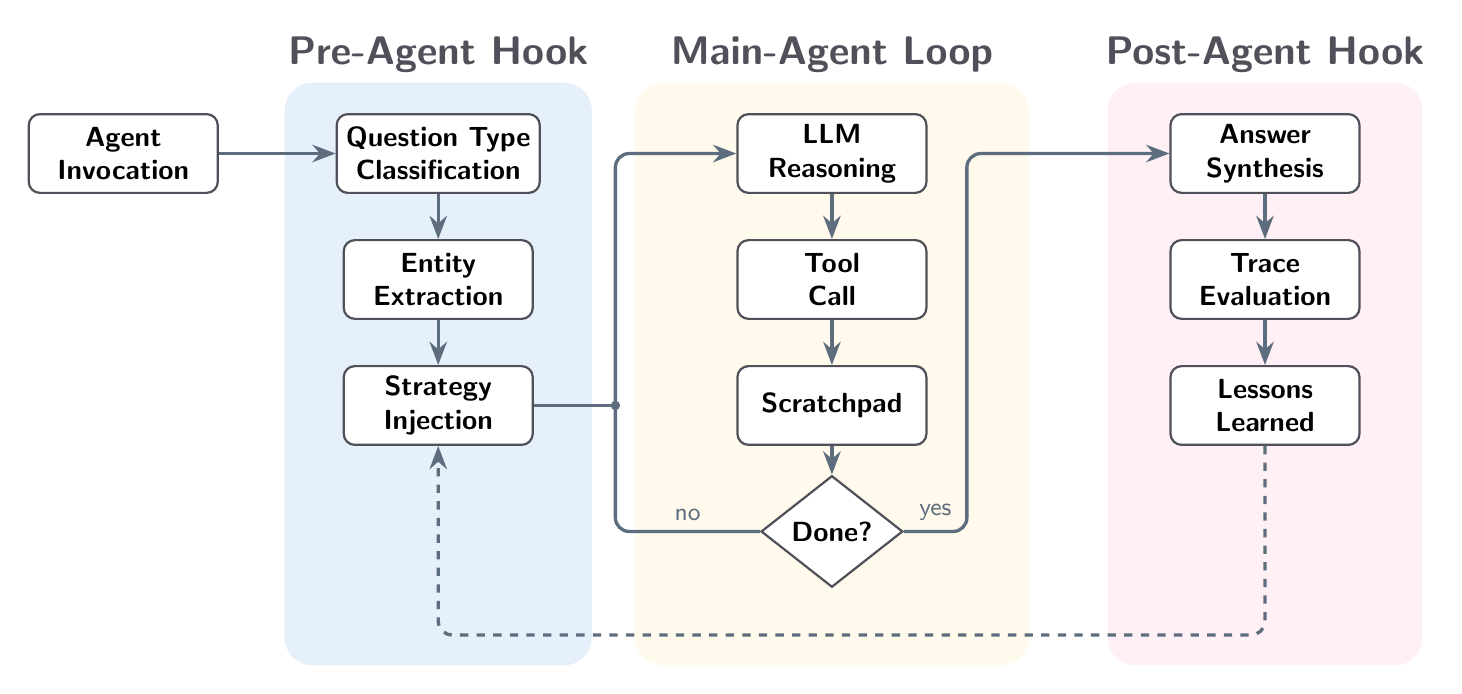
\begin{tikzpicture}[
        >=Stealth,
        %% Grid: y-rows at integer multiples of 1.6; x-columns at fixed centers.
        box/.style={rectangle, rounded corners=4pt, draw=boxgray, thick, fill=white, minimum width=2.4cm, minimum height=1.0cm, align=center, font=\sffamily\normalsize\bfseries},
        widebox/.style={box, minimum width=3.0cm},
        decision/.style={diamond, draw=boxgray, thick, fill=white, minimum width=1.8cm, minimum height=1.4cm, align=center, font=\sffamily\normalsize\bfseries, inner sep=1pt},
        arrow/.style={->, >=Stealth, line width=1.2pt, color=arrowcol, rounded corners=5pt},
        line/.style={color=arrowcol, line width=1.2pt, rounded corners=5pt},
        dasharrow/.style={->, >=Stealth, line width=1.2pt, dashed, color=arrowcol, rounded corners=5pt},
        phaselabel/.style={font=\sffamily\Large\bfseries, text=boxgray}
    ]
    %% --- Starting node (row y=3.2) ---
    \node[box] (user) at (-4.0, 3.2) {Agent\\Invocation};

    %% --- Pre-Agent Hook (top-aligned: rows 3.2, 1.6, 0) ---
    \node[box] (classifier) at (0,  3.2) {Question Type\\Classification};
    \node[box] (extractor)  at (0,  1.6) {Entity\\Extraction};
    \node[box] (strategy)   at (0,  0)   {Strategy\\Injection};

    %% --- Main-Agent Loop (rows 3.2, 1.6, 0, -1.6) ---
    \node[box]    (llm)      at (5.0,  3.2) {LLM\\Reasoning};
    \node[box]    (toolcall) at (5.0,  1.6) {Tool\\Call};
    \node[box]    (result)   at (5.0,  0)   {Scratchpad};
    \node[decision] (done)   at (5.0, -1.6) {Done?};

    %% --- Post-Agent Hook (top-aligned: rows 3.2, 1.6, 0) ---
    \node[box] (synthesis) at (10.5,  3.2) {Answer\\Synthesis};
    \node[box] (judge)     at (10.5,  1.6) {Trace\\Evaluation};
    \node[box] (lessons)   at (10.5,  0)   {Lessons\\Learned};

    %% --- Pre-Agent: sequential top-to-bottom ---
    \draw[arrow] (user.east) -- (classifier.west);
    \draw[arrow] (classifier.south) -- (extractor.north);
    \draw[arrow] (extractor.south)  -- (strategy.north);

    %% --- Shared entry into LLM.west: Done?-no + Strategy share the vertical at x=2.25 ---
    \draw[arrow] (done.west) -- (2.25, -1.6)
        node[midway, above, font=\sffamily\small] {no}
        -- (2.25, 3.2) -- (llm.west);
    \draw[line] (strategy.east) -- (2.25, 0);
    \node[circle, fill=arrowcol, inner sep=1.2pt] at (2.25, 0) {};

    %% --- Main loop internal: top-to-bottom ---
    \draw[arrow] (llm.south)      -- (toolcall.north);
    \draw[arrow] (toolcall.south) -- (result.north);
    \draw[arrow] (result.south)   -- (done.north);

    %% --- Done? "yes" exits east to Post-Agent Hook ---
    \draw[arrow] (done.east) -- ++(0.8, 0)
        node[midway, above, font=\sffamily\small] {yes}
        |- (synthesis.west);

    %% --- Post-Agent flow ---
    \draw[arrow] (synthesis.south) -- (judge.north);
    \draw[arrow] (judge.south)     -- (lessons.north);

    %% --- Feedback: Lessons Learned -> Strategy Injection (dashed, inside bgs, below Done?) ---
    \draw[dasharrow] (lessons.south) -- ++(0, -2.4) -| (strategy.south);

    %% --- Phase backgrounds + labels (compact: 7.4cm tall, centered to keep top headroom) ---
    \begin{scope}[on background layer]
        \node[rectangle, rounded corners=10pt, fill=phasebg1,
              minimum width=3.9cm, minimum height=7.4cm] at (0, 0.4) (bg1) {};
        \node[phaselabel, anchor=south] at (bg1.north) {Pre-Agent Hook};
        \node[rectangle, rounded corners=10pt, fill=phasebg2,
              minimum width=5.0cm, minimum height=7.4cm] at (5.0, 0.4) (bg2) {};
        \node[phaselabel, anchor=south] at (bg2.north) {Main-Agent Loop};
        \node[rectangle, rounded corners=10pt, fill=phasebg3,
              minimum width=4.0cm, minimum height=7.4cm] at (10.5, 0.4) (bg3) {};
        \node[phaselabel, anchor=south] at (bg3.north) {Post-Agent Hook};
    \end{scope}
    \end{tikzpicture}
    }\hfill
    \resizebox{0.44\linewidth}{!}{%
    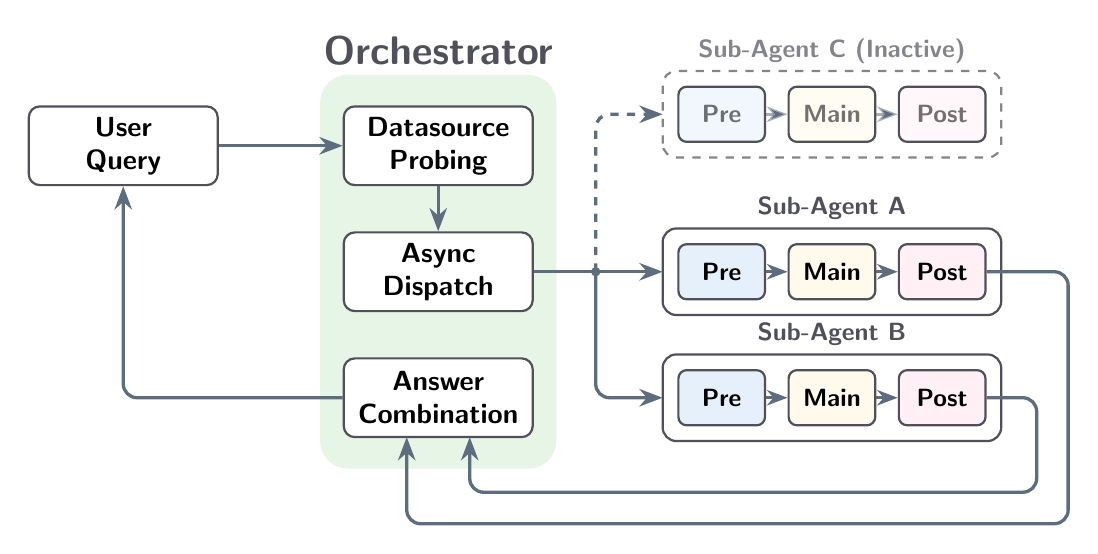
\begin{tikzpicture}[
        >=Stealth,
        box/.style={rectangle, rounded corners=4pt, draw=boxgray, thick, fill=white, minimum width=2.4cm, minimum height=1.0cm, align=center, font=\sffamily\normalsize\bfseries},
        miniPre/.style={rectangle, rounded corners=3pt, draw=boxgray, thick, fill=phasebg1, minimum width=1.1cm, minimum height=0.7cm, align=center, font=\sffamily\small\bfseries},
        miniMain/.style={rectangle, rounded corners=3pt, draw=boxgray, thick, fill=phasebg2, minimum width=1.1cm, minimum height=0.7cm, align=center, font=\sffamily\small\bfseries},
        miniPost/.style={rectangle, rounded corners=3pt, draw=boxgray, thick, fill=phasebg3, minimum width=1.1cm, minimum height=0.7cm, align=center, font=\sffamily\small\bfseries},
        miniarrow/.style={->, >=Stealth, line width=1.0pt, color=arrowcol},
        arrow/.style={->, >=Stealth, line width=1.2pt, color=arrowcol, rounded corners=5pt},
        line/.style={color=arrowcol, line width=1.2pt, rounded corners=5pt},
        dasharrow/.style={->, >=Stealth, line width=1.2pt, dashed, color=arrowcol, rounded corners=5pt},
        phaselabel/.style={font=\sffamily\Large\bfseries, text=boxgray},
        subagentlabel/.style={font=\sffamily\small\bfseries, text=boxgray}
    ]
    \definecolor{phasebgorch}{RGB}{230, 245, 230}

    %% --- User Query ---
    \node[box] (user) at (-4.0, 3.2) {User\\Query};

    %% --- Orchestrator column (rows 3.2, 1.6, 0; same grid step as Fig. 1) ---
    \node[box] (datasource) at (0, 3.2) {Datasource\\Probing};
    \node[box] (async)      at (0, 1.6) {Async\\Dispatch};
    \node[box] (combine)    at (0, 0)   {Answer\\Combination};

    %% --- Sub-Agent C (Inactive, dotted): top, label above container.
    %%     Container expanded with ~0.2 padding around the minis. ---
    \draw[draw=boxgray, thick, dashed, rounded corners=5pt, draw opacity=0.7]
        (2.85, 3.05) rectangle (7.15, 4.15);
    \node[subagentlabel, text opacity=0.7] at (5.0, 4.4) {Sub-Agent C (Inactive)};
    \node[miniPre,  fill opacity=0.55] (cpre)  at (3.6, 3.6) {Pre};
    \node[miniMain, fill opacity=0.55] (cmain) at (5.0, 3.6) {Main};
    \node[miniPost, fill opacity=0.55] (cpost) at (6.4, 3.6) {Post};

    %% --- Sub-Agent A (active), aligned with Async at y=1.6 ---
    \draw[draw=boxgray, thick, rounded corners=5pt]
        (2.85, 1.05) rectangle (7.15, 2.15);
    \node[subagentlabel] at (5.0, 2.4) {Sub-Agent A};
    \node[miniPre]  (apre)  at (3.6, 1.6) {Pre};
    \node[miniMain] (amain) at (5.0, 1.6) {Main};
    \node[miniPost] (apost) at (6.4, 1.6) {Post};

    %% --- Sub-Agent B (active), aligned with Answer Combination at y=0 ---
    \draw[draw=boxgray, thick, rounded corners=5pt]
        (2.85, -0.55) rectangle (7.15, 0.55);
    \node[subagentlabel] at (5.0, 0.8) {Sub-Agent B};
    \node[miniPre]  (bpre)  at (3.6, 0) {Pre};
    \node[miniMain] (bmain) at (5.0, 0) {Main};
    \node[miniPost] (bpost) at (6.4, 0) {Post};

    %% --- Intra-agent arrows ---
    \draw[miniarrow] (apre.east)  -- (amain.west);
    \draw[miniarrow] (amain.east) -- (apost.west);
    \draw[miniarrow] (bpre.east)  -- (bmain.west);
    \draw[miniarrow] (bmain.east) -- (bpost.west);
    \draw[miniarrow, dashed, draw opacity=0.55] (cpre.east)  -- (cmain.west);
    \draw[miniarrow, dashed, draw opacity=0.55] (cmain.east) -- (cpost.west);

    %% --- Orchestrator phase background + label ---
    \begin{scope}[on background layer]
        \node[rectangle, rounded corners=10pt, fill=phasebgorch,
              minimum width=3.0cm, minimum height=5.0cm] at (0, 1.6) (orchbg) {};
        \node[phaselabel, anchor=south] at (orchbg.north) {Orchestrator};
    \end{scope}

    %% --- User -> Orchestrator ---
    \draw[arrow] (user.east) -- (datasource.west);

    %% --- Orchestrator internal flow ---
    \draw[arrow] (datasource.south) -- (async.north);

    %% --- Async dispatch: trunk + 3 branches (A/B solid, C dashed) ---
    \draw[line] (async.east) -- (2.0, 1.6);
    \node[circle, fill=arrowcol, inner sep=1.2pt] at (2.0, 1.6) {};
    \draw[arrow]     (2.0, 1.6) -- (2.85, 1.6);                       %% to A
    \draw[arrow]     (2.0, 1.6) -- (2.0, 0)    -- (2.85, 0);          %% to B (now at y=0)
    \draw[dasharrow] (2.0, 1.6) -- (2.0, 3.6)  -- (2.85, 3.6);        %% to C

    %% --- Returns: A and B exit Post.east, run parallel right + down,
    %%     then enter Combine.south at different x-offsets from below. ---
    \draw[arrow] (apost.east) -- (8.0, 1.6) -- (8.0, -1.6) -- (-0.4, -1.6) -- (-0.4, -0.5);
    \draw[arrow] (bpost.east) -- (7.6, 0.0) -- (7.6, -1.2) -- ( 0.4, -1.2) -- ( 0.4, -0.5);

    %% --- Loop back: Combine -> User ---
    \draw[arrow] (combine.west) -| (user.south);

    \end{tikzpicture}
    }
    \caption{Left: agent lifecycle, with deterministic pre-processing,
    an iterative tool-calling main loop over a scratchpad, and post-hoc
    synthesis, trace evaluation, and lesson distillation. Right: the
    multi-agent orchestrator dispatches the question to the sub-agents
    matched by the routing probe (each an instance of the left
    lifecycle) and merges their grounded answers; unmatched sub-agents
    stay inactive.}
    \label{fig:arch}
\end{figure}


\paragraph{Agent lifecycle.}
Each sub-agent runs the same three-phase lifecycle
(Fig.~\ref{fig:arch}, left). A deterministic pre-agent hook classifies
the question by type and extracts candidate entities, injecting a
matching strategy document and type-specific few-shot examples into
the system prompt. The main loop then iteratively calls typed tools
and writes its findings to a structured
scratchpad~\cite{nye2021scratchpad} of visited nodes, discovered
values, and verified facts; deterministic comparison and
verification tools offload numeric and boolean logic from the language
model, and a loop detector injects recovery guidance when the agent
stalls. Finally, a post-agent hook synthesises the answer solely from
the scratchpad's verified facts, and a judging agent scores the trace
so that good runs become few-shot examples for future queries.

\paragraph{Access control by design.}
Since every knowledge-graph interaction passes through deterministic
SPARQL wrappers, access policy can be enforced at a single, auditable
boundary: each typed tool can inject named-graph filters or row-level
predicates derived from the caller's identity before a query reaches
the triple store, which is more verifiable than prompt-based
restrictions; enforcing such policies is future work.

\paragraph{KG onboarding.}
A hierarchy of dataclasses declares everything the reasoning core
needs to know about a graph: Uniform Resource Identifier (URI)
prefixes, endpoint and named-graph
settings, reification and temporal-data flags, and vector-collection
bindings. Onboarding a new KG follows four steps. (1)~The RDF dump is
loaded into the triple store under a dedicated named graph.
(2)~Entity labels and relation names are indexed into two vector
collections, powering fuzzy entry-point discovery and the routing
probe. (3)~\texttt{BaseKGAdapter} is subclassed to return the
populated configuration, and the graph is exposed through an MCP
server that implements the abstract tool interface as
endpoint-specific SPARQL templates. (4)~The new sub-agent, which
declares only its adapter and MCP-server path, is registered with the
orchestrator. Both reference integrations are a few hundred lines of
largely declarative code; an unseen graph can typically be onboarded
in a few hours.

\smallskip\noindent\textbf{Evaluation excerpt.}
Table~\ref{tab:eval} reports representative results with an
open-weights backbone: 84\% on the Wikidata-derived KQAPro
benchmark~\cite{cao2022kqapro} and, through its own adapter without
core changes, 73\% on the SciQA benchmark~\cite{sciqa2023} over the
Open Research Knowledge Graph (ORKG).

\begin{table}[t]
  \caption{Evaluation excerpt: 100 sampled questions per dataset,
  per-question averages. At public per-token rates a question stays
  below \$0.04.}
  \label{tab:eval}
  \centering
  \begin{tabular}{llrrr}
    \toprule
    Dataset & LLM & Accuracy & Avg. time & Avg. tokens\\
    \midrule
    KQAPro & Gemma4-31B & 84\% & 30.8\,s & 69.4\,k\\
    SciQA  & Gemma4-31B & 73\% & 37.5\,s & 129.7\,k\\
    \bottomrule
  \end{tabular}
\end{table}

\section{Demonstration}
At our demo booth, attendees pick an agent (the Orchestrator by
default, or a KQAPro/SciQA specialist with stateful multi-turn
follow-ups) and a backbone LLM. While the agent runs, the UI animates
the lifecycle of Fig.~\ref{fig:arch} (left) live, and in Orchestrator
mode the swarm view of Fig.~\ref{fig:demo}: stages light up as their
trace spans open, and the routing probe's per-source evidence feeds an
explicit \texttt{select\_agent} decision. Once the answer arrives
(Fig.~\ref{fig:demo}, left), a Trace tab exposes the full trace as a
span tree, down to individual LLM messages, tool calls, and the raw
SPARQL issued.

\begin{figure}[tb]
  \centering
  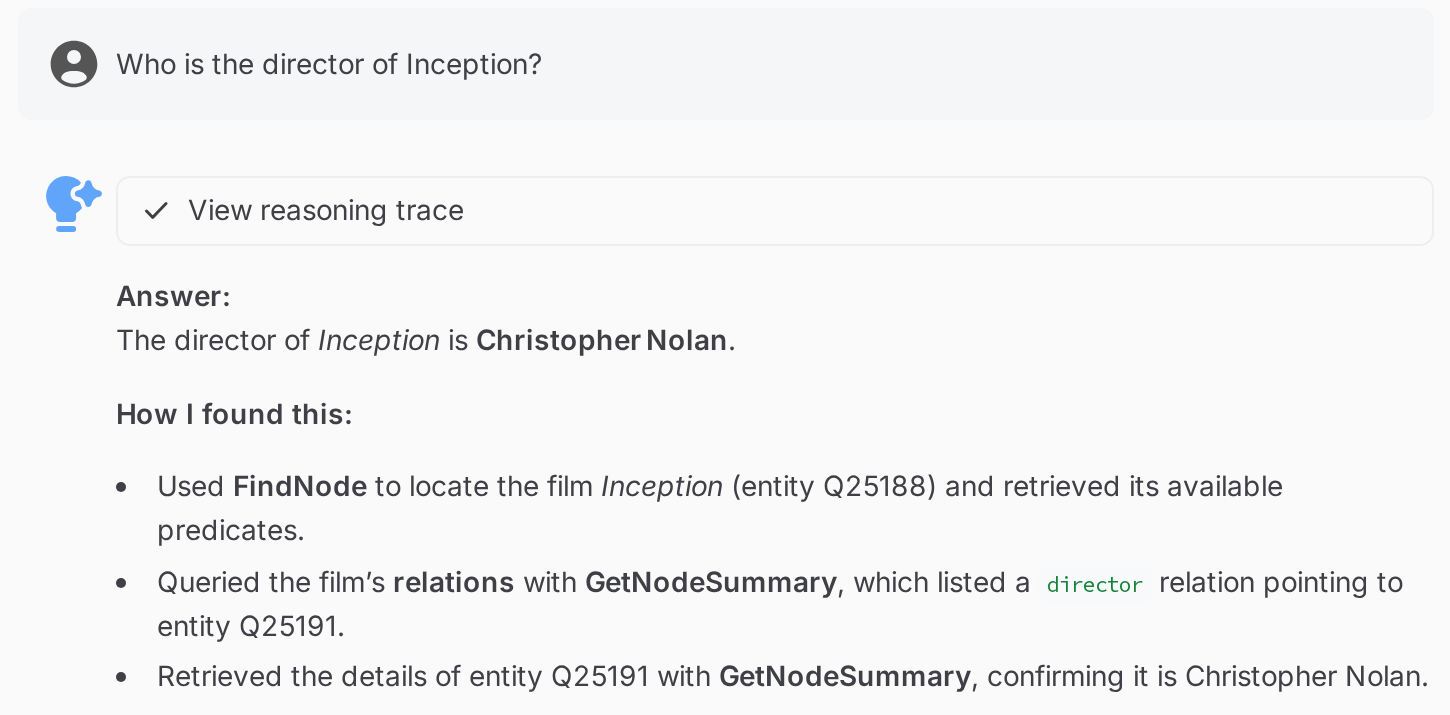
\includegraphics[width=0.445\linewidth]{figures/demo_answer.png}\hfill
  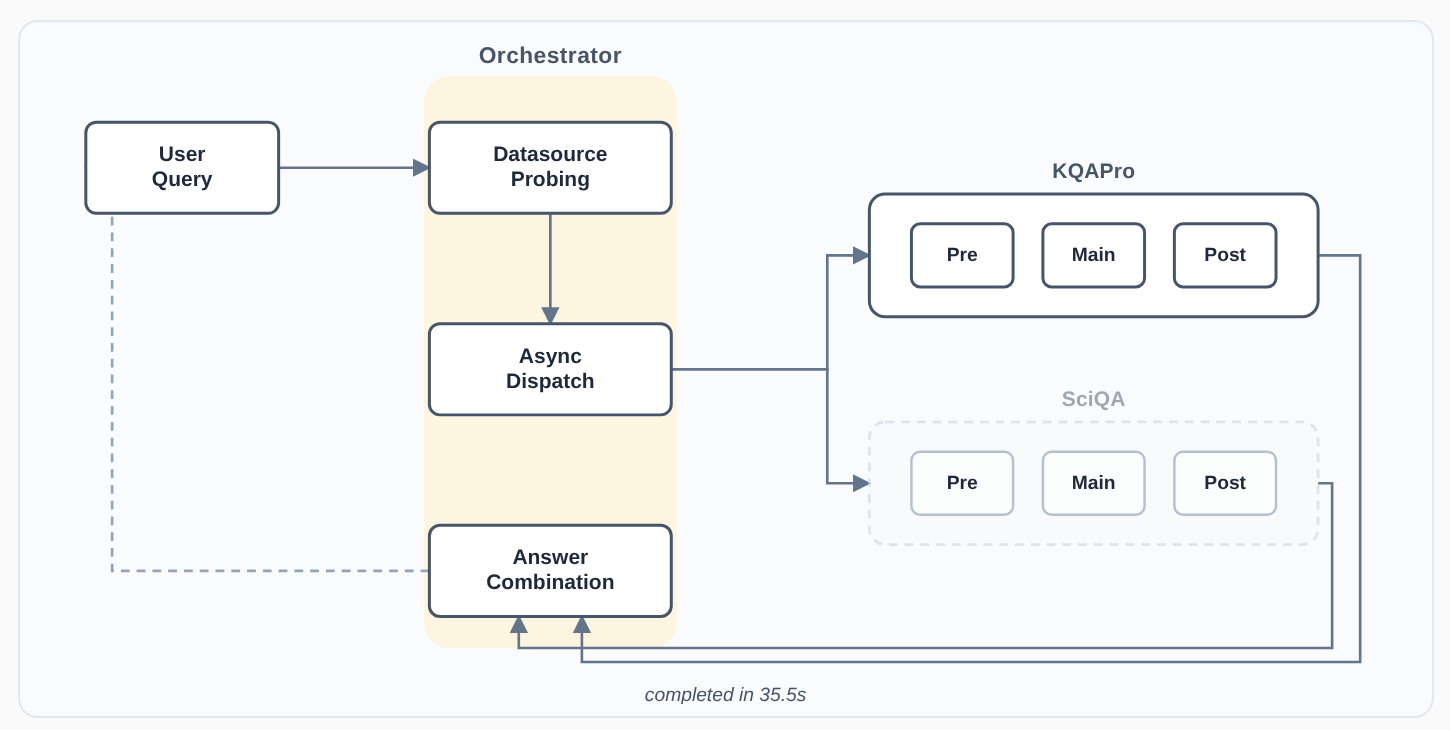
\includegraphics[width=0.41\linewidth]{figures/demo_lifecycle.png}
  \caption{The demo answering a question via the Orchestrator. Left:
  the grounded answer cites the tool calls behind each step. Right:
  the live swarm view; the probe matched KQAPro, so only that
  sub-agent animates while SciQA stays inactive.}
  \label{fig:demo}
\end{figure}

\section{Conclusion}
We showcased AMA-KBQA, a functional prototype of a training-free
multi-agent system for KBQA over heterogeneous RDF graphs. A single
reasoning core with per-graph MCP SPARQL-wrapper tools reaches
competitive accuracy on KQAPro and ports to SciQA without any change
to the core (Table~\ref{tab:eval}), at practical runtimes and costs.
Accuracy on SciQA still trails KQAPro's, automated onboarding remains
open, and the wrapper boundary is designed for per-caller access
control that we have yet to enforce; we see these as promising
directions towards a portable, model-agnostic KBQA ecosystem.

\section*{Acknowledgments}
This work was carried out in the Seminar Knowledge Discovery at KIT's AIFB institute and supported by the Deutsche Forschungsgemeinschaft (DFG) under Research Unit FOR 5339 (Project No.459291153).

\section*{Declaration on Generative AI}
The authors used Claude for grammar and spelling checks, paraphrasing, and implementation assistance; the LLMs inside AMA-KBQA are themselves the object of study. Generative AI was not used to conceive the research idea, make architectural decisions, formulate the evaluation, or draw conclusions. The authors reviewed and edited all code and content and take full responsibility for it.

\bibliography{references}

\end{document}
